\documentclass[a0paper,portrait]{baposter}

\usepackage{wrapfig}
\usepackage{lmodern}

\usepackage[utf8]{inputenc} %unicode support
\usepackage[T1]{fontenc}
\usepackage[dvipsnames]{xcolor}
\usepackage[most]{tcolorbox}
\usepackage{color,soul}
\usepackage{tikz}
\usepackage{multirow}
\usepackage{booktabs}
\usepackage{url}
\usepackage{enumitem}
\usepackage{caption}

\usepackage{graphicx}           % \includegraphics
\usepackage{tcolorbox}          % cajas
\usepackage{xcolor}             % colores
\usepackage{array}              % >{\raggedright\arraybackslash}p{...}
\usepackage{booktabs}
\usepackage{caption}
\usepackage{float}

\definecolor{lightgreen}{HTML}{E3FAE3}
\definecolor{blue}{HTML}{C3D6EF}
\definecolor{pale}{HTML}{E4C3B6}
\definecolor{violet}{HTML}{DECBE8}
\sethlcolor{violet}

\graphicspath{{figures/}} % Directory in which figures are stored

\newcommand{\compresslist}{%
\setlength{\itemsep}{0pt}%
\setlength{\parskip}{1pt}%
\setlength{\parsep}{0pt}%
}
\definecolor{lightorange}{RGB}{0,70,220}  % color de cabeceras

\newenvironment{boenumerate}
  {\begin{enumerate}\renewcommand\labelenumi{\textbf\theenumi.}}
  {\end{enumerate}}

\begin{document}

% --- tamaños compactos ---
\newcommand{\TitleLineA}{\fontsize{22}{26}\selectfont\sffamily\bfseries}
\newcommand{\TitleLineB}{\fontsize{18}{22}\selectfont\sffamily\bfseries}
\newcommand{\AuthorsLine}{\normalsize\sffamily}
\newcommand{\AffilLine}{\footnotesize\sffamily}

% Loro Twemoji (U+1F99C) del paper. Es la página 2707 de all-twemojis.pdf del
% paquete twemojis, extraída como PDF suelto para no depender del paquete.
% Reflejado, igual que en el paper. Emojis (c) Twitter Inc. y otros, CC-BY 4.0.
% Separación entre el loro y la C de Chatty. Va en negativo porque el PDF del
% emoji trae su propio margen transparente: con 0em el hueco sigue siendo ancho.
% Con el loro delante (ver \ChattyTitle): -0.20em roza, -0.35em pico sobre la C,
% -0.50em el loro monta sobre la C y sigue leyéndose, -0.65em la tapa casi entera.
\newcommand{\ParrotGap}{-0.35em}
\newcommand{\parrotemoji}{\raisebox{-0.25em}{\reflectbox{
\includegraphics[height=0.92em]{figures/parrot.pdf}}}}

% El título se compone en dos pasos para que el loro quede POR DELANTE de las
% letras: primero se reserva su hueco y se escribe el texto, y después se repinta
% el loro encima con \llap (ancho cero, así la línea conserva su anchura). En el
% orden natural la C tapa al loro en cuanto \ParrotGap hace que se solapen.
\newsavebox{\parrotbox}
\newsavebox{\chattybox}
\newcommand{\ChattyTitle}{%
  \sbox{\parrotbox}{\parrotemoji}%
  \sbox{\chattybox}{Chatty:}%
  \kern\wd\parrotbox
  \kern\ParrotGap
  \usebox{\chattybox}%
  \llap{\usebox{\parrotbox}\kern\dimexpr\ParrotGap+\wd\chattybox\relax}%
}

% Anchos de los logos de financiación (banda inferior), como fracción del ancho de
% la caja. Ojo: baposter compone la página a fontscale=0.31 y la escala x3.23, así
% que una longitud absoluta (cm) NO es la del A0 impreso; por eso se dimensionan en
% fracciones de \linewidth. Suman 0.93: el 0.07 restante son los dos huecos que
% reparte \hfill, de modo que la fila queda justificada a todo el ancho.
% Alturas impresas resultantes: ~4.9 / 4.3 / 4.0 cm. La 3 lleva más ancho que las
% otras porque su marca es más apaisada y, a igual altura, se vería más pequeña.
\newcommand{\FundWA}{0.319\linewidth}   % MICIU + Cofinanciado UE + AEI
\newcommand{\FundWB}{0.228\linewidth}   % Xunta de Galicia
\newcommand{\FundWC}{0.383\linewidth}   % Cátedra CAMELIA
\newcommand{\FundLogo}[2]{\raisebox{-0.5\height}{\includegraphics[width=#1]{#2}}}

% Card para figuras con título arriba
\tcbset{
  figurecard/.style={
    enhanced,
    sharp corners,
    colback=white,
    colframe=black!12,
    boxrule=0.4pt,
    arc=6pt,
    left=2pt, right=2pt, top=10pt, bottom=8pt,
    fonttitle=\bfseries\sffamily,
    attach boxed title to top left={yshift=-2.0mm, xshift=0.6em},
    halign title=left,
    boxed title style={
      colback=lightorange, colframe=lightorange,
      boxrule=0pt, arc=3pt,
      sharp corners,
      top=2pt, bottom=2pt, left=8pt, right=8pt
    },
    valign=top
  }
}

\tcbset{
  infocard/.style={
    enhanced,
    sharp corners,
    colback=white,
    colframe=black!12,
    boxrule=0.4pt,
    arc=6pt,
    left=4pt, right=4pt, top=7pt, bottom=5pt,
    fonttitle=\bfseries\sffamily,
    attach boxed title to top left={yshift=-2.0mm, xshift=0.6em},
    halign title=left,
    boxed title style={
      colback=lightorange, colframe=lightorange,
      boxrule=0pt, arc=3pt,
      sharp corners,
      top=2pt, bottom=2pt, left=8pt, right=8pt
    },
    valign=top
  }
}

\tcbset{
  resultcard/.style={
    enhanced,
    colback=white,
    colframe=black!10,
    boxrule=0.4pt,
    sharp corners=all,
    left=4pt,right=4pt,top=4pt,bottom=4pt,
    boxsep=2pt,
    fonttitle=\bfseries,
    title filled,
    colbacktitle=black!2,
    coltitle=black
  },
}

\begin{poster}{
  grid=false,
  headerborder=none,
  colspacing=1em,
  bgColorOne=white,
  bgColorTwo=white,
  borderColor=white,
  headerColorOne=lightorange,
  headerColorTwo=lightorange,
  headerFontColor=white,
  boxColorOne=white,
  textborder=rounded,
  eyecatcher=false,
  headerheight=0.133\textheight,
  headershape=rounded,
  headershade=plain,
  headerfont=\Large\sffamily,
  textfont=\normalsize\sffamily,
  linewidth=1.4pt
}{}
% -------------------- IZQUIERDA (vacío) --------------------
{}
% -------------------- CENTRO (Título + Autores) --------------------
{
  \makebox[\linewidth][l]{%
    \hspace{0.2cm}
    \parbox{1.0\linewidth}{\raggedright
      {\TitleLineA \ChattyTitle}\\[0.2em]
      {\TitleLineB A Tool for Building and Evaluating Customizable LLM Assistants}\\[0.4em]
      {\AuthorsLine Manuel Couto-Pintos, Marcos Fernández-Pichel, Mario Ezra Aragón, David Gallego-Conde, and David E. Losada}\\
      {\AffilLine Centro Singular de Investigación en Tecnoloxías Intelixentes (CiTIUS), Universidade de Santiago de Compostela (USC), Spain}\\
      {\AffilLine\texttt{\{manuel.couto.pintos, marcosfernandez.pichel, ezra.aragon, davidgallego.conde, david.losada\}@usc.es}}
    }%
  }
}
% -------------------- DERECHA (Logos) --------------------
{
  \begin{minipage}{0.3\linewidth}
  \centering
  \raggedleft
  
\includegraphics[width=0.6\linewidth]{figures/logo_citius.png}
  \hspace{0.25cm}
\end{minipage}
}

% -------------------- 1. WHAT IS CHATTY? (col 0-1, span 2) --------------------
\headerbox{}{name=intro,column=0,span=2,row=0,
  headerColorOne=white, headerColorTwo=white, headerFontColor=white,
  headerborder=none, textborder=none, boxColorOne=white}{
  \vspace{-1.0cm}

  \begin{tcolorbox}[infocard, title={1. What is Chatty?}]
    \noindent
    \begin{minipage}[c]{0.47\linewidth}
      \small
      \textbf{Chatty} customizes Large Language Model (LLM) assistants through structured \textbf{role biasing}.

      \vspace{15pt}
      A library of predefined \textbf{system roles} and prompt templates instantiates assistants with distinct behaviors, across \textbf{multiple LLM families}.

      \vspace{15pt}
      A \textbf{parallel chat} interface enables synchronous, side-by-side comparison of completions; conversations can be downloaded or frozen.

      \vspace{15pt}
      Useful for research in \textbf{conversational AI} and \textbf{LLM evaluation}, and for building conversational datasets.
    \end{minipage}\hfill
    \begin{minipage}[c]{0.51\linewidth}
      \centering
      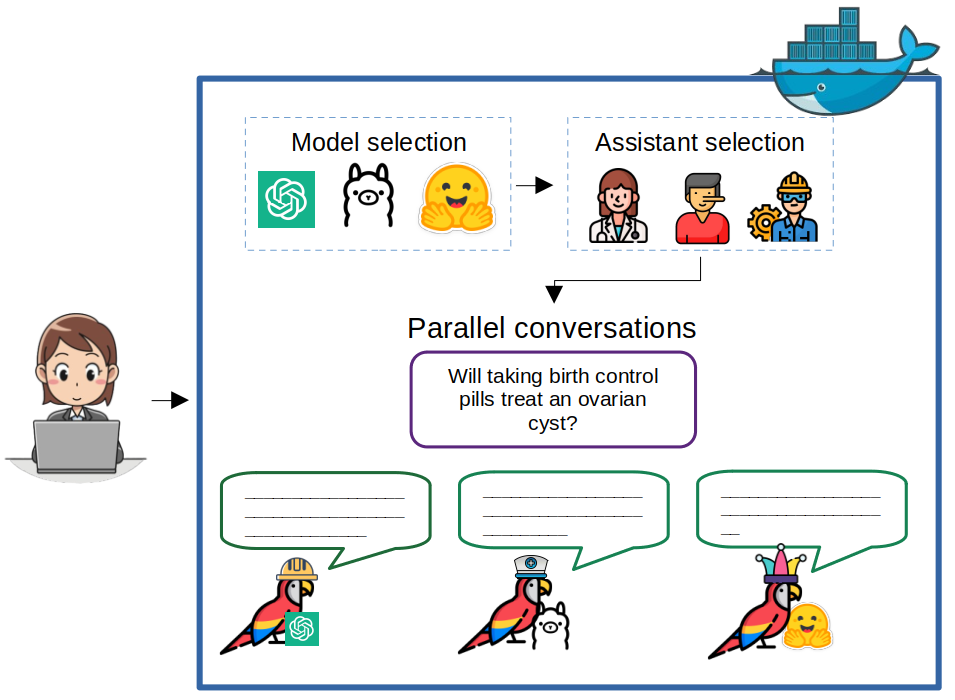
\includegraphics[width=\linewidth]{figures/chatty_overview.png}
    \end{minipage}
  \end{tcolorbox}
}

% -------------------- 2. CONTRIBUTIONS (col 2, span 1) --------------------
\headerbox{}{name=contrib,column=2,span=1,row=0,
  headerColorOne=white, headerColorTwo=white, headerFontColor=white,
  headerborder=none, textborder=none, boxColorOne=white}{
  \vspace{-1.0cm}

  \begin{tcolorbox}[infocard, title={2. Contributions}]
    \begin{minipage}[t]{\linewidth}
      \small
      \begin{itemize}\itemsep10pt \parskip0pt \parsep0pt \leftskip-0.4cm
        \item A versatile, reusable \textbf{role-customization library}: tailor assistants through model selection, persona definition and specialized prompt configurations.
        \item A structured conversational interface that seamlessly connects assistant prompts and \textbf{LLM families}, enabling role-based biases and prompt suggestions.
        \item Facilitates the creation of \textbf{synthetic conversational datasets} for research in LLM evaluation, conversational AI, bias detection and multi-model collaboration.
        \item A \textbf{health-misinformation} use case that exemplifies comparing assistant outputs in a highly strategic, high-stakes domain.
      \end{itemize}
    \end{minipage}
  \end{tcolorbox}
}

% -------------------- 3. SYSTEM ARCHITECTURE (col 0-1, span 2) --------------------
\headerbox{}{name=system,span=2,column=0,below=intro,
  headerColorOne=white, headerColorTwo=white, headerFontColor=white,
  headerborder=none, textborder=none, boxColorOne=white}{
  \vspace{-1.0cm}

  \begin{tcolorbox}[figurecard, title={3. System Architecture \& Implementation}]
    \noindent
    \begin{minipage}[c]{0.44\linewidth}
      \centering
      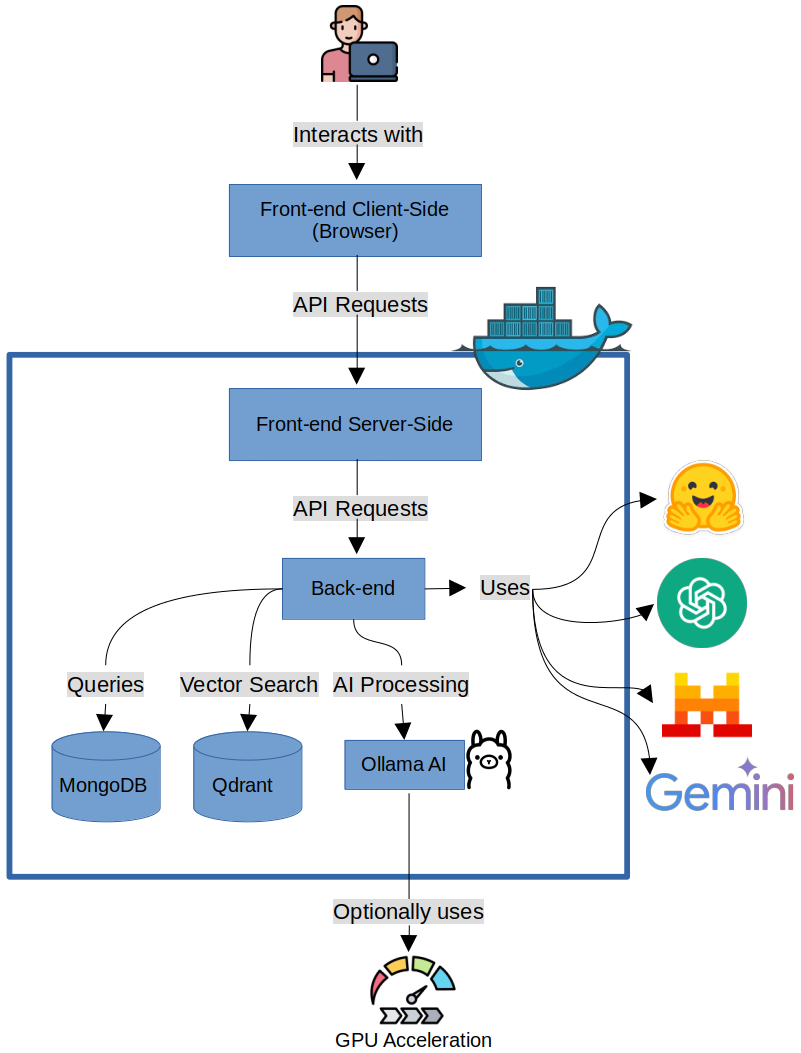
\includegraphics[width=\linewidth]{figures/chatty_architecture.png}
    \end{minipage}\hfill
    \begin{minipage}[c]{0.54\linewidth}
      \begin{tcolorbox}[resultcard, title={Three-layer design (containerized)}]
        \small
        \begin{itemize}\itemsep2pt \parskip0pt \parsep0pt \leftskip-0.4cm
          \item \textbf{UI (front-end):} browser interface to pick models, configure roles, enter prompts and compare responses.
          \item \textbf{Back-end (Docker):} handles queries, vector search and AI processing via API.
          \item \textbf{Models \& storage:} MongoDB (sessions/prompts), Qdrant (vector search), LLMs via Hugging Face, OpenAI, Mistral, Gemini and Ollama; optional GPU.
        \end{itemize}
      \end{tcolorbox}
      \vspace{0.3em}
      \begin{tcolorbox}[resultcard, title={Functionalities}]
        \small
        \begin{itemize}\itemsep2pt \parskip0pt \parsep0pt \leftskip-0.4cm
          \item Multi-model support and \textbf{role-based biasing}.
          \item Up to \textbf{4 parallel completions} chatted synchronously.
          \item Conversation management: download logs (CSV/JSON), synchronize, freeze.
          \item \textbf{One-click} containerized deployment (deployed on a local 5090 GPU, 32\,GB VRAM).
        \end{itemize}
      \end{tcolorbox}
    \end{minipage}
  \end{tcolorbox}
}

% -------------------- 4. MODELS & ROLES (col 2, span 1) --------------------
\headerbox{}{name=modelroles,span=1,column=2,below=contrib,
  headerColorOne=white, headerColorTwo=white, headerFontColor=white,
  headerborder=none, textborder=none, boxColorOne=white}{
  \vspace{-1.0cm}

  \begin{tcolorbox}[infocard, title={4. Models \& Assistant Roles}]
    \small
    \begin{itemize}\itemsep10pt \parskip0pt \parsep0pt \leftskip-0.4cm
      \item \textbf{Multiple LLM families:} GPT-4/3, Flan-T5, Gemma3, Llama3, \ldots, served through OpenAI, Hugging Face, Anthropic, Mistral, Gemini and local Ollama models (quantized to reduce latency).
      \item \textbf{More than 100 predefined assistant roles} (Doctor, Debater, Screenwriter, \ldots), plus user-defined custom prompts.
      \item Selecting a \textbf{model + role} instantiates an assistant; the role tailors its behavior and response style, streamlining prompt engineering for novices and experts.
      \item Each model--role configuration is added as a vertical block, enabling direct side-by-side comparison of completions.
    \end{itemize}
  \end{tcolorbox}
}

% -------------------- 5. CASE STUDY (col 0-1, span 2) --------------------
\headerbox{}{name=casestudy,span=2,column=0,below=system,
  headerColorOne=white, headerColorTwo=white, headerFontColor=white,
  headerborder=none, textborder=none, boxColorOne=white}{
  \vspace{-1.0cm}

  \begin{tcolorbox}[infocard, title={5. Case Study: Health Misinformation}]
    \noindent
    \begin{minipage}[c]{0.50\linewidth}
      \small
      An expert \textbf{psychologist} evaluated Chatty on \textbf{50 health questions} from the TREC 2021 Health Misinformation Track (yes/no ground truth = medical consensus).

      \vspace{3pt}
      Three assistants built on \textbf{GPT-3} were compared:
      \begin{itemize}\itemsep2pt \parskip0pt \parsep0pt \leftskip-0.4cm
        \item \textbf{Neutral} -- receives only the question.
        \item \textbf{Liar} -- designed to introduce inaccuracies.
        \item \textbf{Doctor} -- expert-level medical assistant.
      \end{itemize}
    \end{minipage}\hfill
    \begin{minipage}[c]{0.47\linewidth}
      \begin{tcolorbox}[resultcard, title={Evaluation criteria (expert)}]
        \small
        \begin{itemize}\itemsep2pt \parskip0pt \parsep0pt \leftskip-0.4cm
          \item \textbf{Q1} -- alignment with medical consensus.
          \item \textbf{Q2} -- comprehension of the query.
          \item \textbf{Q3} -- relevance \& factuality.
          \item \textbf{Q4} -- misleading content.
        \end{itemize}
      \end{tcolorbox}
    \end{minipage}
  \end{tcolorbox}
}

% -------------------- 6. RESULTS (col 2, span 1) --------------------
\headerbox{}{name=results,span=1,column=2,below=modelroles,
  headerColorOne=white, headerColorTwo=white, headerFontColor=white,
  headerborder=none, textborder=none, boxColorOne=white}{
  \vspace{-1.0cm}

  \begin{tcolorbox}[infocard, title={6. Results}]
    \centering
    \begin{tcolorbox}[resultcard, title={Q1 -- Alignment with medical consensus}]
      \centering
      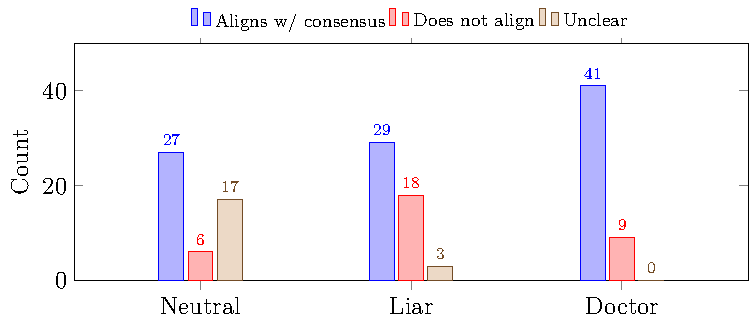
\includegraphics[width=0.70\linewidth]{figures/chart_q1.pdf}
    \end{tcolorbox}
    \vspace{0.22em}
    \begin{tcolorbox}[resultcard, title={Q3 -- Relevance \& factuality}]
      \centering
      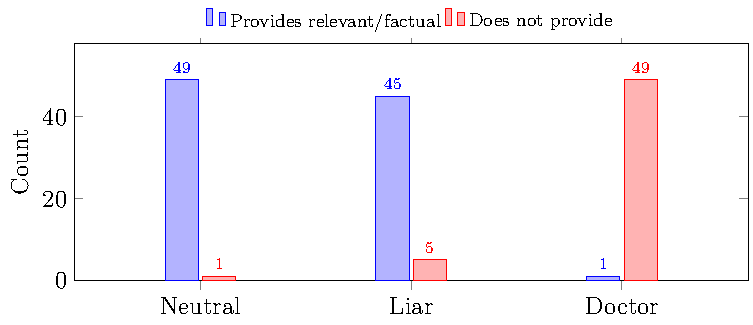
\includegraphics[width=0.70\linewidth]{figures/chart_q3.pdf}
    \end{tcolorbox}
    \vspace{0.22em}
    \begin{tcolorbox}[resultcard, title={Key observations}]
      \small \raggedright
      \begin{itemize}\itemsep4pt \parskip0pt \parsep0pt \leftskip-0.4cm
        \item \textbf{Q1:} the \textbf{Doctor} assistant is the most aligned with medical consensus (\textbf{41/50} correct), highlighting the value of specialized roles.
        \item \textbf{Q2:} all assistants showed perfect comprehension of the questions, regardless of the provided context.
        \item \textbf{Q3:} the \emph{Neutral} role gave more explicit factual information, whereas the \emph{Doctor} tended to short yes/no answers.
        \item \textbf{Q4:} no assistant produced offensive or harmful content.
      \end{itemize}
    \end{tcolorbox}
  \end{tcolorbox}
}

% -------------------- Try it & Resources (QRs) — LEFT (col 0) --------------------
\headerbox{}{name=qr,span=1,column=0,below=casestudy,
  headerColorOne=white, headerColorTwo=white, headerFontColor=white,
  headerborder=none, textborder=none, boxColorOne=white}{
  \vspace{-1.0cm}
  \begin{tcolorbox}[infocard, title={Try it \& Resources}]
    \noindent
    \begin{minipage}[c]{0.49\linewidth}
      \centering
      
\includegraphics[width=0.56\linewidth]{figures/qr_github.png}\\[3pt]
      {\small Code \& quick start}
    \end{minipage}\hfill
    \begin{minipage}[c]{0.49\linewidth}
      \centering
      
\includegraphics[width=0.56\linewidth]{figures/qr_video.png}\\[3pt]
      {\small Video demo}
    \end{minipage}
  \end{tcolorbox}
}

% -------------------- SEPLN logo — LEFT, below the QRs (outside any card) --------------------
\headerbox{}{name=footer,span=1,column=0,below=qr,
  headerColorOne=white, headerColorTwo=white, headerFontColor=white,
  headerborder=none, textborder=none, boxColorOne=white}{
  \vspace{-0.7cm}
  \begin{center}
    
\includegraphics[width=0.50\linewidth]{figures/sepln2026_logo.png}
  \end{center}
}

% -------------------- 7. KEY FINDINGS & CONCLUSIONS — MIDDLE (col 1, span 1), aligned with Try it --------------------
\headerbox{}{name=conclusions,span=1,column=1,below=casestudy,
  headerColorOne=white, headerColorTwo=white, headerFontColor=white,
  headerborder=none, textborder=none, boxColorOne=white}{
  \vspace{-1.0cm}

  \begin{tcolorbox}[infocard, title={7. Key Findings \& Conclusions}]
    \small
    \begin{itemize}\itemsep4pt \parskip0pt \parsep0pt \leftskip-0.4cm
      \item \textbf{Domain-specific role prompting} (e.g., a medical Doctor role) substantially improves the reliability of AI-generated content.
      \item System-role instructions strongly \textbf{shape model behavior}; the \emph{Neutral} role cites more factual detail, while the \emph{Doctor} tends to short yes/no answers.
      \item The \emph{Liar} role is convincing yet wrong, exemplifying the \textbf{misinformation risk} of advanced generation.
      \item Current effectiveness is \textbf{insufficient without expert supervision} in high-stakes domains such as healthcare.
      \item \textbf{Future work:} adaptive role switching and multilingual capabilities.
    \end{itemize}
  \end{tcolorbox}
}

% -------------------- FINANCIACIÓN — fila única a todo lo ancho, al pie --------------------
\headerbox{}{name=funding,span=3,column=0,below=conclusions,
  headerColorOne=white, headerColorTwo=white, headerFontColor=white,
  headerborder=none, textborder=none, boxColorOne=white}{
  \vspace{-1.15cm}
  {\parindent0pt
    \FundLogo{\FundWA}{figures/logo1.png}\hfill
    \FundLogo{\FundWB}{figures/logo2.png}\hfill
    \FundLogo{\FundWC}{figures/logo3.png}%
    \par}
}

\end{poster}

\end{document}
